\section{Event-B XText Front-end Overview}
\label{sec:overview}

The Event-B XText Front-end provides new XEvent-B constructs (XMachines and XContexts) which are text files which are automatically translated into the corresponding Rodin Event-B constructs (i.e., Machine and Context) accordingly.  Facility for translating from Rodin Event-B components to XEvent-B components can be invoked manually. The overall process can be seen in Figure~\ref{fig:overview}.
\begin{figure}[!htbp]
  \centering
  \ifplastex
  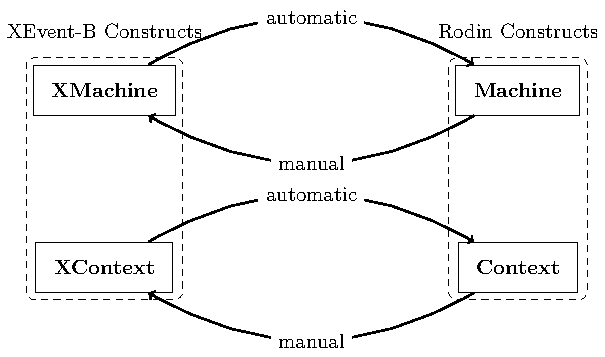
\includegraphics[width=512]{tikz-overview}
  \else
  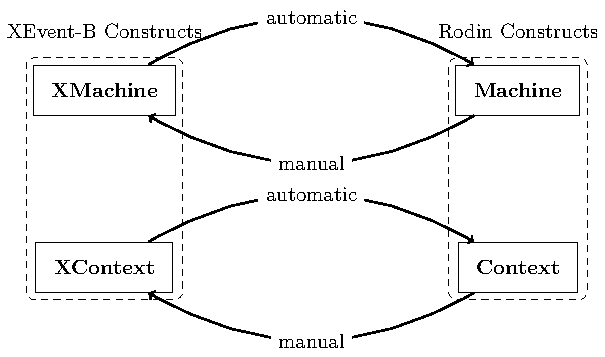
\includegraphics[width=0.9\textwidth]{tikz-overview}
  \fi
  \caption{Overview of XEvent-B and Rodin Event-B Constructs}
  \label{fig:overview}
\end{figure}

%%% Local Variables:
%%% mode: latex
%%% TeX-master: "user_manual"
%%% End:
